% !TEX encoding = UTF-8
% !TEX TS-program = pdflatex
% !TEX root = ../tesi.tex

%**************************************************************
\chapter{Analisi del problema}
\label{cap:analisi-del-problema}
%**************************************************************

\intro{In questo capitolo vengono elencati e descritti i casi d’uso emersi durante la fase di analisi del software precedente e del prodotto sviluppato, e mostrato, tramite opportune tabelle, il tracciamento dei requisiti.}\\

%**************************************************************
\section{Cos'è un web crawler?}

Un web crawler è un software che analizza i contenuti di una rete in un modo metodico e automatizzato. L'utilizzo più comune dei crawler avviene sul World Wide Web; tramite una lista di URL da visitare identifica tutti i collegamenti ipertestuali presenti nel documento e li aggiunge alla lista di URL da visitare. Data la natura della ricerca essa potrebbe protrarsi per un tempo indefinito, tuttavia, grazie ad alcune politiche si può influenzare l'ordine di ricerca, la frequenza e quali pagine evitare. I motori di ricerca odierni si basano su web crawler per poter ricercare ed indicizzare i vari siti internet.

\begin{figure}[!h] 
    \centering 
    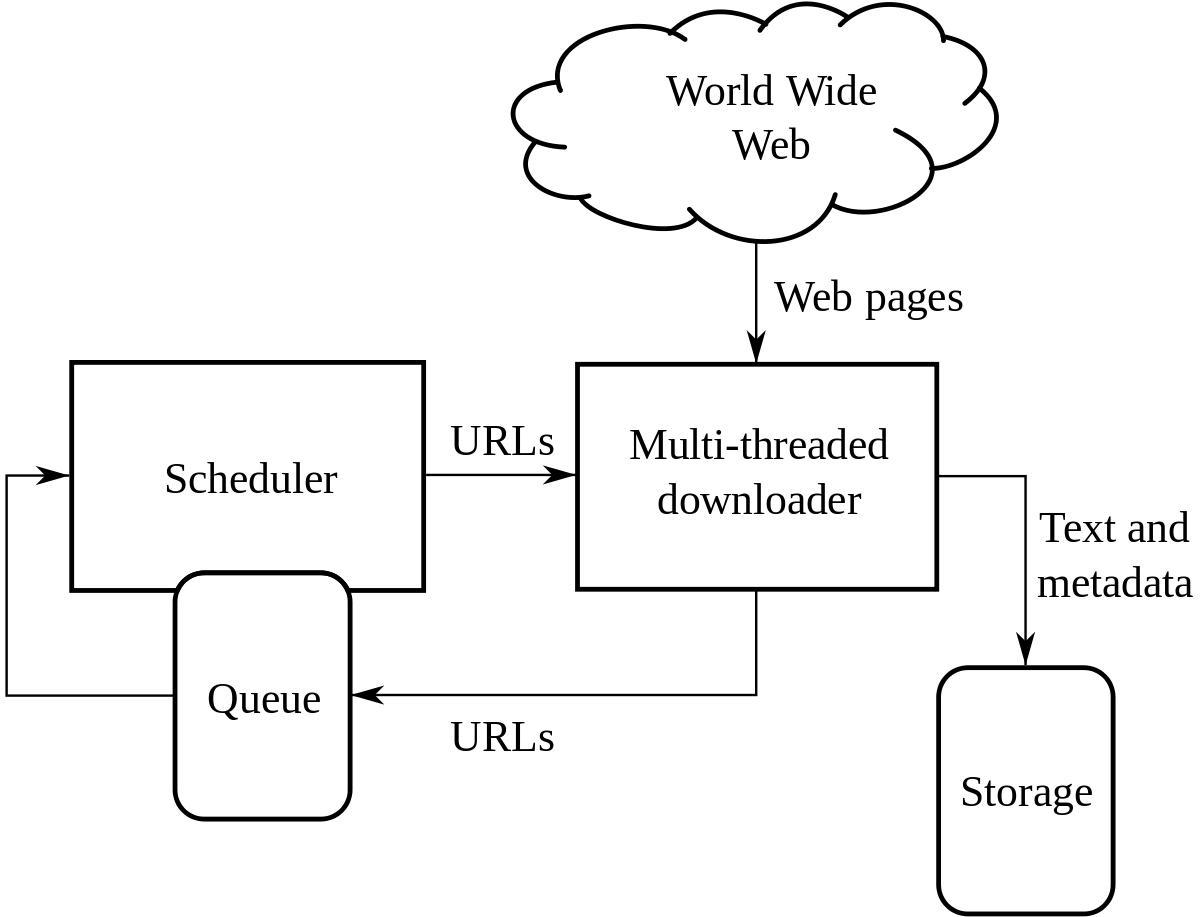
\includegraphics[width=0.3\columnwidth]{WebCrawlerArchitecture.png} 
    \caption{Architettura di un web crawler.}
\end{figure}

%**************************************************************
\section{Cosa significa web scraping?}

Con il termine web scraping ci si riferisce all'estrapolazione di dati dai siti web. Il termine generalmente comprende anche l'estrapolazione fatta manualmente tramite software anche se il termine principalmente si riferisce al processo automatizzato implementato tramite web crawler. L'attività principale di cui si occupa un web scraper è la trasformazione di informazioni libere in informazioni strutturate per renderle di più facile utilizzo per una successiva analisi. 

\begin{figure}[!h] 
    \centering 
    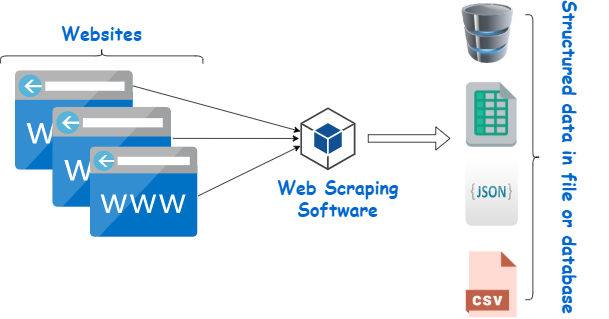
\includegraphics[width=0.3\columnwidth]{webscraping.png} 
    \caption{Funzionamento di un web scraper.}
\end{figure}

%**************************************************************

\section{Studio dei moduli presenti}

Prima di progettare e sviluppare il nuovo modulo di web crawling, ho effettuato un’analisi della struttura della piattaforma presente per comprenderne la struttura e le funzionalità offerte. Principalmente è stato fondamentale individuare l'organizzazione delle funzionalità di log, l'organizzazione dei file di configurazione e il codice principale da cui si avvia il programma. La struttura del modulo è risultata pulita, di facile comprensione e molto scalabile, richiedendo per l'inserimento del nuovo modulo l'aggiunta di poche e coincise linee di codice.


\section{Individuazione delle funzionalità}

Il modulo di web crawling e web scraping oltre a rispettare le definizioni date in precedenza deve rispettare delle funzionalità ritenute obbligatorie. Innanzitutto per poter navigare il dark web deve essere possibile effettuare chiamate di rete tramite la rete Tor. In seguito vista la grande mole di dati prevista durante l'attività di crawling, deve essere fornita al programma una serie di politiche per poter correttamente individuare le priorità delle singole pagine portando ad una più veloce individuazione delle risorse ritenute fondamentali. Al fine di garantire un corretto mantenimento e utilizzo del modulo, deve essere implementato un sistema di log delle informazioni e degli errori. Infine, anche se non era stato richiesto obbligatoriamente, il prodotto software è stato sviluppato per essere indipendente dal sistema operativo utilizzato.


\subsection{Funzionalità aggiuntive}

%**************************************************************
\section{Caratteristiche del modulo}
%**************************************************************